\documentclass[UTF8,a4paper,12pt]{ctexart}
\usepackage[left=2.25cm,right=2.25cm,top=2.45cm,bottom=2.85cm]{geometry}
\usepackage{amsmath,amssymb,bm}
\usepackage{booktabs,array,longtable,multirow}
\usepackage{graphicx}
\usepackage{float}
\usepackage{xcolor}
\usepackage{caption}
\usepackage{subcaption}
\usepackage{enumitem}
\usepackage{hyperref}
\usepackage{fancyhdr}
\hypersetup{colorlinks=true,linkcolor=black,urlcolor=blue,citecolor=black}
\captionsetup{font=small,labelsep=quad}
\setlength{\parindent}{2em}
\setlength{\parskip}{0.25em}
\linespread{1.18}
\renewcommand{\arraystretch}{1.18}
\setlength{\footskip}{1.15cm}
\pagestyle{fancy}
\setlength{\headheight}{15pt}
\fancyhf{}
\fancyhead[C]{多波束测深覆盖模型与测线优化设计}
\fancyfoot[C]{\thepage}
\renewcommand{\headrulewidth}{0.4pt}
\graphicspath{{../../诊断结果/Q03/}{../../诊断结果/Q04/}}
\newcommand{\nmi}{\,\mathrm{nmi}}
\newcommand{\m}{\,\mathrm{m}}
\newcommand{\km}{\,\mathrm{km}}
\newcommand{\degree}{^\circ}

\title{\heiti 多波束测深覆盖模型与测线优化设计}
\author{匿名}
\date{}

\begin{document}
\maketitle

\begin{abstract}
针对平面斜坡和历史网格地形上的多波束测深覆盖与测线规划问题，本文建立由二维射线—斜面、三维方向投影、区间并集和分片地形共同组成的统一模型。第一问在恒定坡度剖面内推导左右覆盖宽度与有向重叠率；当测线位置由 $-800\m$ 移至 $800\m$ 时，水深由 $90.95\m$ 降至 $49.05\m$，坡面覆盖宽度由 $315.81\m$ 降至 $170.33\m$，后两组正式重叠率为 $-1.39\%$ 和 $-11.17\%$，表明出现漏测。第二问把海底梯度分别投影到测线沿向和横向，得到任意方向下的解析覆盖模型，并以完整三维射线—平面求交复核 64 个结果；覆盖宽度范围为 $62.90$--$768.48\m$，双实现最大绝对差为 $5.6843\times10^{-13}\m$。第三问在直线平行设计类中沿等深线由深水侧向浅水侧递推变间距，得到 34 条南北向测线，总长度 $125.936\km$，正式重叠率为 $10.01\%$，全区域无漏测；相较 $15\%$ 基线缩短 $5.56\%$。第四问以历史水深网格的分片双线性面为主地形，按“漏测率—过度重叠长度—总长度”的分层目标比较九个实际候选，最终采用南北分块的 86 条直线，总长度 $473.186\km$；$5\m$ 主评价下漏测率为 0，重叠率超过 $20\%$ 的逐对计数线段总长为 $131.287\km$。人工地形、独立射线求交、二维栅格并集、分辨率细化和两种三角剖分均支持所得结论。本文同时明确：第3、4问的最优性限于实际计算的直线候选类，数值离散差异不构成真实设备或海底变化的物理误差保证。

\textbf{关键词：}多波束测深；射线—平面求交；覆盖宽度；有向重叠率；测线优化；规则网格地形
\end{abstract}

\tableofcontents
\newpage

\section{问题重述}

多波束测深系统以竖直中心波束和两侧边界波束形成扇形探测面。海底坡度使两侧覆盖不对称，测线方向和位置又会改变有效横向坡度及水深。题目依次要求：在二维恒坡剖面中填写表水深、覆盖宽度和相邻重叠；建立任意有向测线方向的三维覆盖模型并完成 64 个组合；在 $4\nmi\times2\nmi$ 恒坡矩形海域中设计满足完整覆盖与 $10\%$--$20\%$ 重叠的短测线；最后根据 $4\nmi\times5\nmi$ 历史水深网格设计测线，并评价漏测面积比例、重叠率超过 $20\%$ 的相关线段总长度和区域内测线总长度。

\section{问题分析}

四问具有递进结构：第一问给出二维基本几何和重叠口径；第二问把坡度投影到任意测线的横断面；第三问把单条覆盖区间扩展为恒坡矩形上的区间并集与变间距递推；第四问用数据驱动的分片地形替代恒坡，并把覆盖评价提升到二维区域测度。

求解采用三层结构：先推导可核查的闭式几何，再用区间并集或分片地形生成具体测线，最后冻结方案并使用不参与调参的独立求交、栅格和地形表示进行确认。这一结构保留了解析可解释性，也避免仅凭中心间距公式声称全区域覆盖。

\section{模型假设}

\begin{enumerate}[leftmargin=2.6em]
  \item 换能器中心波束竖直向下，边界波束关于中心波束对称，总开角为 $\theta$，半开角为 $\gamma=\theta/2$。
  \item 问题1--3使用题面给出的 $\theta=120\degree$；问题4采用用户批准的同一开角作为规划基准，而非将其写成第4问题面事实。
  \item 问题1--3的海底按题面恒坡面处理；问题4以附件历史水深网格为规划基准，主模型采用分片双线性面。
  \item 忽略声速折射、波束厚度、船体姿态、定位误差与设备标定误差。
  \item 问题3、4的总长度只计待测区域内部有效段，不计转场、转弯、港口往返和区域外连接。
  \item 问题3采用前一条带宽度归一的有向重叠率；问题4沿用该口径识别超过 $20\%$ 的线段。
  \item 可行性判断使用未舍入数，舍入只发生在论文表格和结果工作簿显示层。
\end{enumerate}

\section{符号说明}

\begin{table}[H]
\centering
\caption{主要符号}
\begin{tabular}{clc}
\toprule
符号 & 含义 & 单位\\
\midrule
$\theta,\gamma$ & 总开角、半开角，$\gamma=\theta/2$ & 度或弧度\\
$\beta$ & 第2问起的有向测线方向角 & 度或弧度\\
$\alpha$ & 恒坡海底坡度角 & 度或弧度\\
$D_0,D_i$ & 中心水深、位置 $i$ 的垂直水深 & m\\
$x,y,z$ & 东、北、上方向坐标 & m\\
$q$ & 恒坡剖面上的有向弧长坐标 & m\\
$m_\perp$ & 测线横向的有向高程坡度 & 1\\
$L_i,R_i,W_i$ & 条带左右边界、覆盖宽度 & m\\
$S_i,O_i,G_i$ & 有符号重叠、实际交长、漏测间隙 & m\\
$\eta_i$ & 以前一条带宽度归一的重叠率 & 1\\
$A_{\rm miss},p_{\rm miss}$ & 漏测面积、漏测面积比例 & $\mathrm{m}^2$, \%\\
$L_{\eta>20\%}$ & 重叠率超过20\%的逐对计数线段总长 & m\\
\bottomrule
\end{tabular}
\end{table}

\section{第1问：二维恒坡覆盖与重叠}

\subsection{坡面、水深与边界波束}

取水平 $x$ 轴向东上坡，竖直 $z$ 轴向上。海底坡面及位置 $x_i$ 的水深为
\begin{equation}
z=-D_0+x\tan\alpha,\qquad D_i=D_0-x_i\tan\alpha.
\end{equation}

两条边界射线与坡面相交后，下坡侧和上坡侧的坡面距离分别为
\begin{equation}
a_i=\frac{D_i\sin\gamma}{\cos(\gamma+\alpha)},\qquad
b_i=\frac{D_i\sin\gamma}{\cos(\gamma-\alpha)}.
\end{equation}

在坡面弧长坐标 $q=x/\cos\alpha$ 中，
\begin{equation}
I_i=[L_i,R_i]=[q_i-a_i,q_i+b_i],
\end{equation}
\begin{equation}
W_i=D_i\sin\gamma\left[
\frac{1}{\cos(\gamma+\alpha)}+
\frac{1}{\cos(\gamma-\alpha)}
\right].
\end{equation}

\subsection{有向重叠率}

相邻条带的有符号重叠、实际交长和漏测间隙为
\begin{equation}
S_i=\min(R_{i-1},R_i)-\max(L_{i-1},L_i),
\end{equation}
\begin{equation}
O_i=\max(0,S_i),\qquad G_i=\max(0,-S_i).
\end{equation}
正式重叠率取
\begin{equation}
\eta_i=\frac{S_i}{W_{i-1}}.
\end{equation}
它保留负值表示漏测，并在平坦、等宽情形恢复 $\eta=1-d/W$。

\subsection{结果与验证}

给定 $D_0=70\m$、$\alpha=1.5\degree$、$\theta=120\degree$，计算结果见表\ref{tab:q1}。

\begin{table}[H]
\centering
\caption{第1问正式结果}
\label{tab:q1}
\resizebox{\textwidth}{!}{
\begin{tabular}{lrrrrrrrrr}
\toprule
距中心距离/m & -800&-600&-400&-200&0&200&400&600&800\\
\midrule
水深/m &90.95&85.71&80.47&75.24&70.00&64.76&59.53&54.29&49.05\\
覆盖宽度/m &315.81&297.63&279.44&261.26&243.07&224.88&206.70&188.51&170.33\\
与前线重叠率/\% &--&33.64&29.59&25.00&19.78&13.78&6.81&-1.39&-11.17\\
\bottomrule
\end{tabular}}
\end{table}

在 $600\m$ 和 $800\m$ 处分别出现约 $2.875\m$ 与 $21.061\m$ 的漏测间隙。独立参数射线—直线求交的最大长度差为 $1.1369\times10^{-13}\m$；平坦极限、坡向镜像、区间边界例与工作簿读回均通过。

\section{第2问：任意方向的三维覆盖}

\subsection{坐标与有效横向坡度}

取 $x$ 轴向东上坡、$y$ 轴向北、$z$ 轴向上。海底平面仍为 $z=-D_0+x\tan\alpha$。依题图取坡面法向量水平投影的西侧下坡方向为 $\beta=0\degree$，正角从 $+z$ 观察逆时针。测线沿向与左横向单位向量为
\begin{equation}
\bm u_\beta=(-\cos\beta,-\sin\beta,0),\qquad
\bm q_\beta=(\sin\beta,-\cos\beta,0).
\end{equation}
正距离 $d$ 表示船从海域中心沿 $\bm u_\beta$ 前进。船位水深及横向有效坡度为
\begin{equation}
D(\beta,d)=D_0+d\tan\alpha\cos\beta,
\end{equation}
\begin{equation}
m_{\rm eff}=\tan\alpha\sin\beta,\qquad
\alpha_{\rm eff}=\arctan m_{\rm eff}.
\end{equation}
坡面覆盖宽度为
\begin{equation}
W=D\sin\gamma\left[
\frac{1}{\cos(\gamma+\alpha_{\rm eff})}+
\frac{1}{\cos(\gamma-\alpha_{\rm eff})}
\right].
\end{equation}

\subsection{64个正式结果}

给定 $D_0=120\m$、$\alpha=1.5\degree$，表\ref{tab:q2} 的列为距离（海里），表内为覆盖宽度（米）。

\begin{table}[H]
\centering
\caption{第2问任意方向覆盖宽度}
\label{tab:q2}
\resizebox{\textwidth}{!}{
\begin{tabular}{rrrrrrrrr}
\toprule
$\beta/\degree$ &0&0.3&0.6&0.9&1.2&1.5&1.8&2.1\\
\midrule
0&415.69&466.09&516.49&566.89&617.29&667.69&718.09&768.48\\
45&416.19&451.87&487.55&523.23&558.91&594.59&630.27&665.95\\
90&416.69&416.69&416.69&416.69&416.69&416.69&416.69&416.69\\
135&416.19&380.51&344.83&309.15&273.47&237.79&202.11&166.43\\
180&415.69&365.29&314.89&264.50&214.10&163.70&113.30&62.90\\
225&416.19&380.51&344.83&309.15&273.47&237.79&202.11&166.43\\
270&416.69&416.69&416.69&416.69&416.69&416.69&416.69&416.69\\
315&416.19&451.87&487.55&523.23&558.91&594.59&630.27&665.95\\
\bottomrule
\end{tabular}}
\end{table}

独立验证令边界射线方向为
\begin{equation}
\bm d_\pm=\pm\sin\gamma\,\bm q_\beta-\cos\gamma\,\bm e_z,
\end{equation}
直接与海底平面求交，再由两端点的三维距离求宽度。64 个组合的最大绝对差为 $5.6843\times10^{-13}\m$，最大相对差为 $2.6719\times10^{-15}$。方向对称、反向航向、平坦极限、单位换算和 Excel 读回均通过。

\section{第3问：恒坡矩形的测线优化}

\subsection{方向选择与递推}

矩形东西宽 $4\nmi$、南北长 $2\nmi$。等深线沿南北方向，因此南北向测线上的水深恒定。东西向坡向测线在同一条线上跨越全部水深，按中心条件给出的统一间距会在深水侧产生超过 $20\%$ 的重叠、在浅水侧产生漏测，故不可行。

在坡面坐标中记
\begin{equation}
A=\frac{\sin\gamma}{\cos(\gamma+\alpha)},\qquad
B=\frac{\sin\gamma}{\cos(\gamma-\alpha)}.
\end{equation}
第 $i$ 条带为
\begin{equation}
I_i=[q_i-AD_i,\ q_i+BD_i].
\end{equation}
首条线令左边界恰达西边界，其后取目标重叠率 $\eta_0=0.1001$，按
\begin{equation}
L_i=R_{i-1}-\eta_0W_{i-1}
\end{equation}
逐条求取最东可行位置，末条覆盖东边界。

\subsection{方案与验证}

最终得到 34 条南北向平行线，每条区域内长度为 $3704\m$。首条横坐标为 $-3345.4782\m$，末条为 $3684.9455\m$。水深从 $197.6044\m$ 降至 $13.5063\m$，相邻间距从 $589.2744\m$ 降至 $43.6886\m$。总长度
\begin{equation}
L_3=34\times3704=125936\m=125.936\km.
\end{equation}

\begin{figure}[H]
\centering
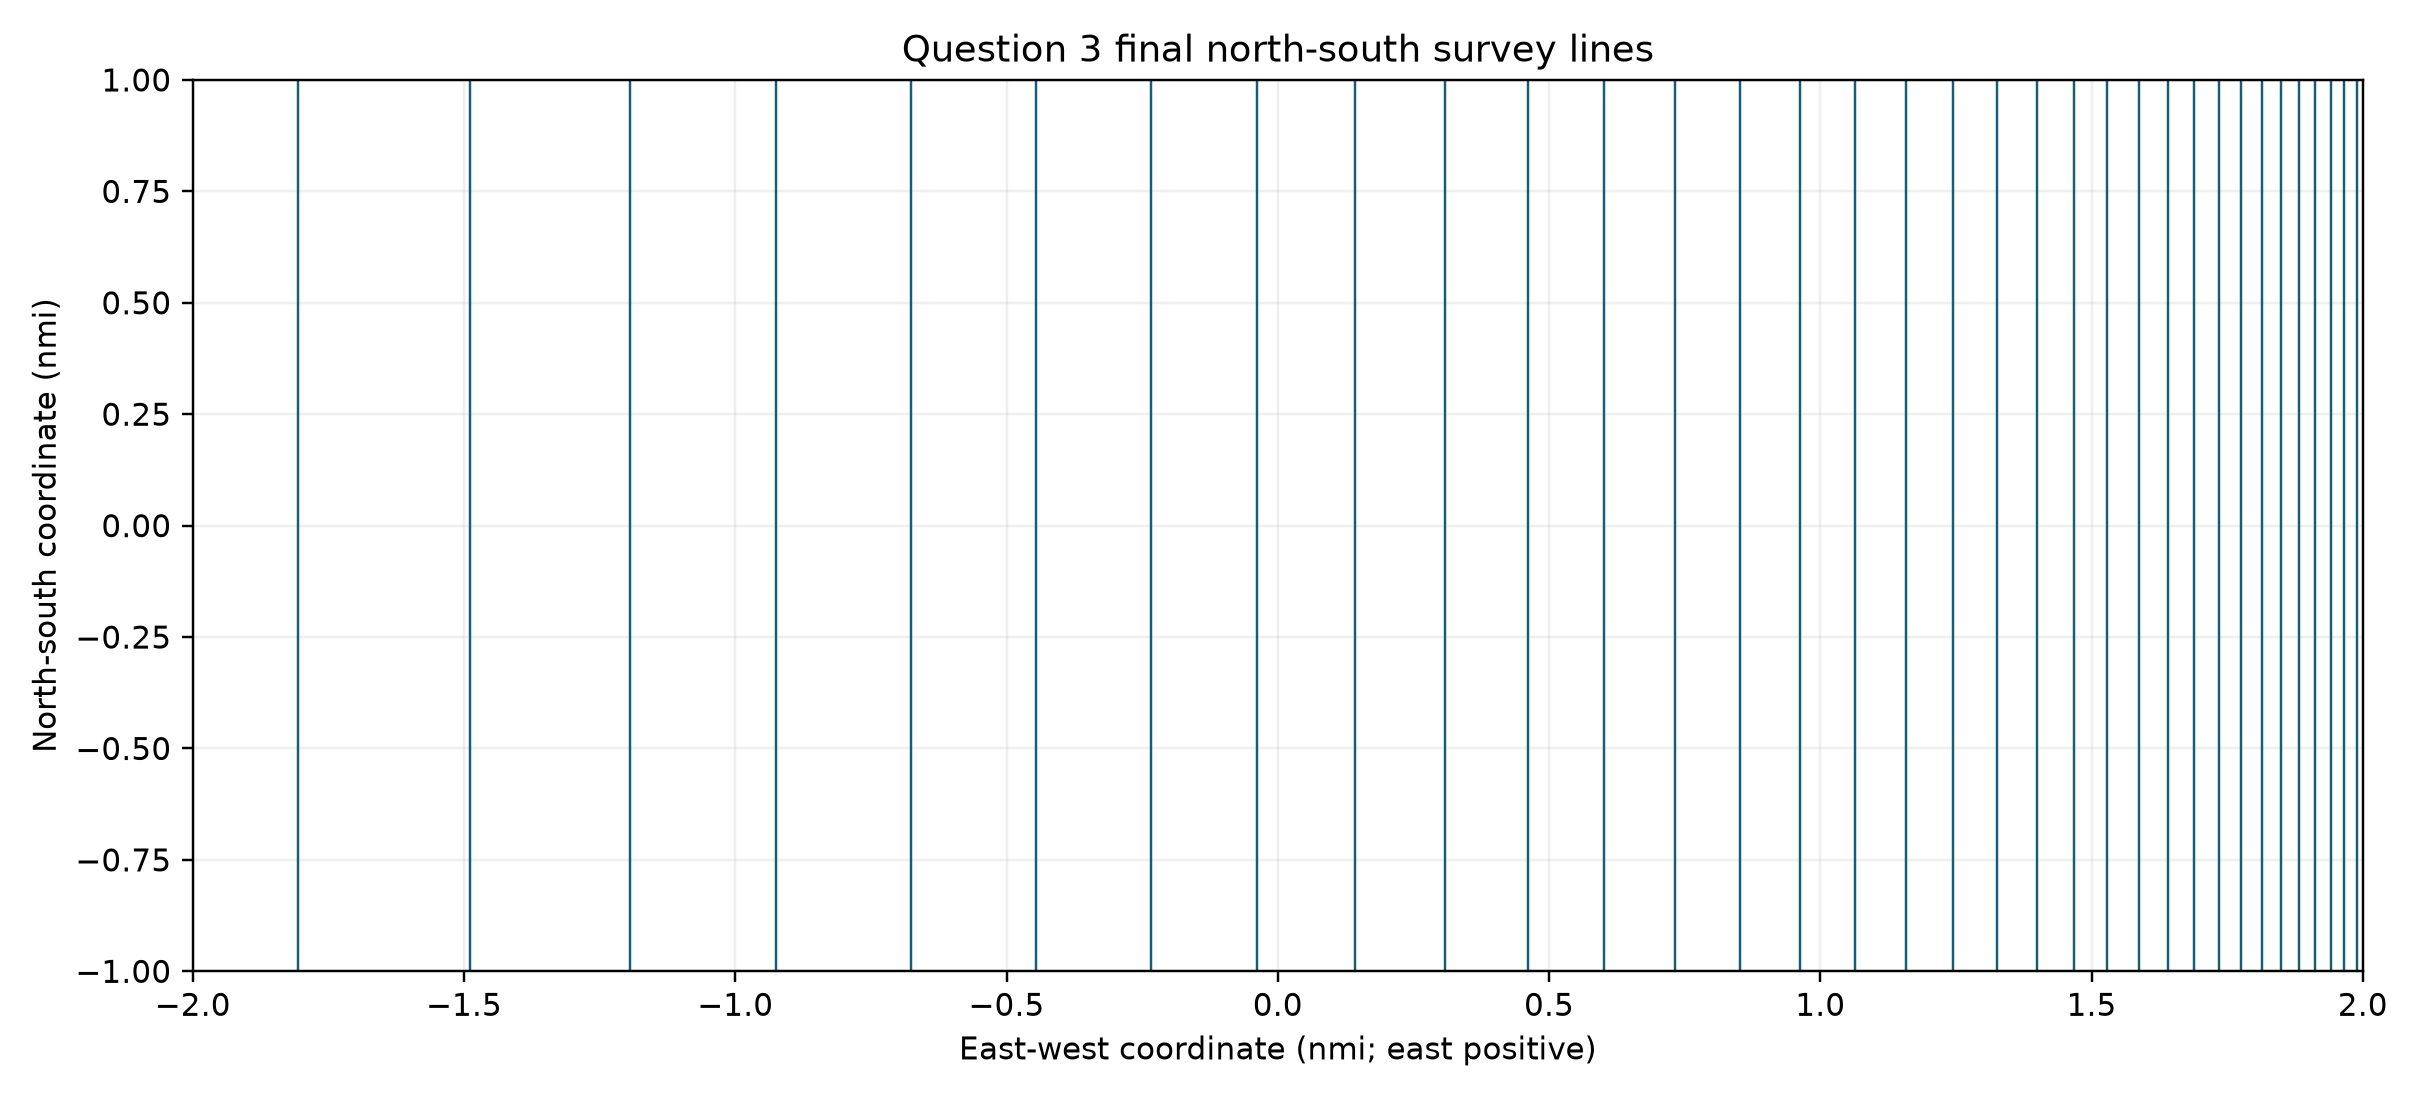
\includegraphics[width=0.88\textwidth]{第3问测线布局-v001.png}
\caption{第3问最终测线布局}
\label{fig:q3layout}
\end{figure}

\begin{figure}[H]
\centering
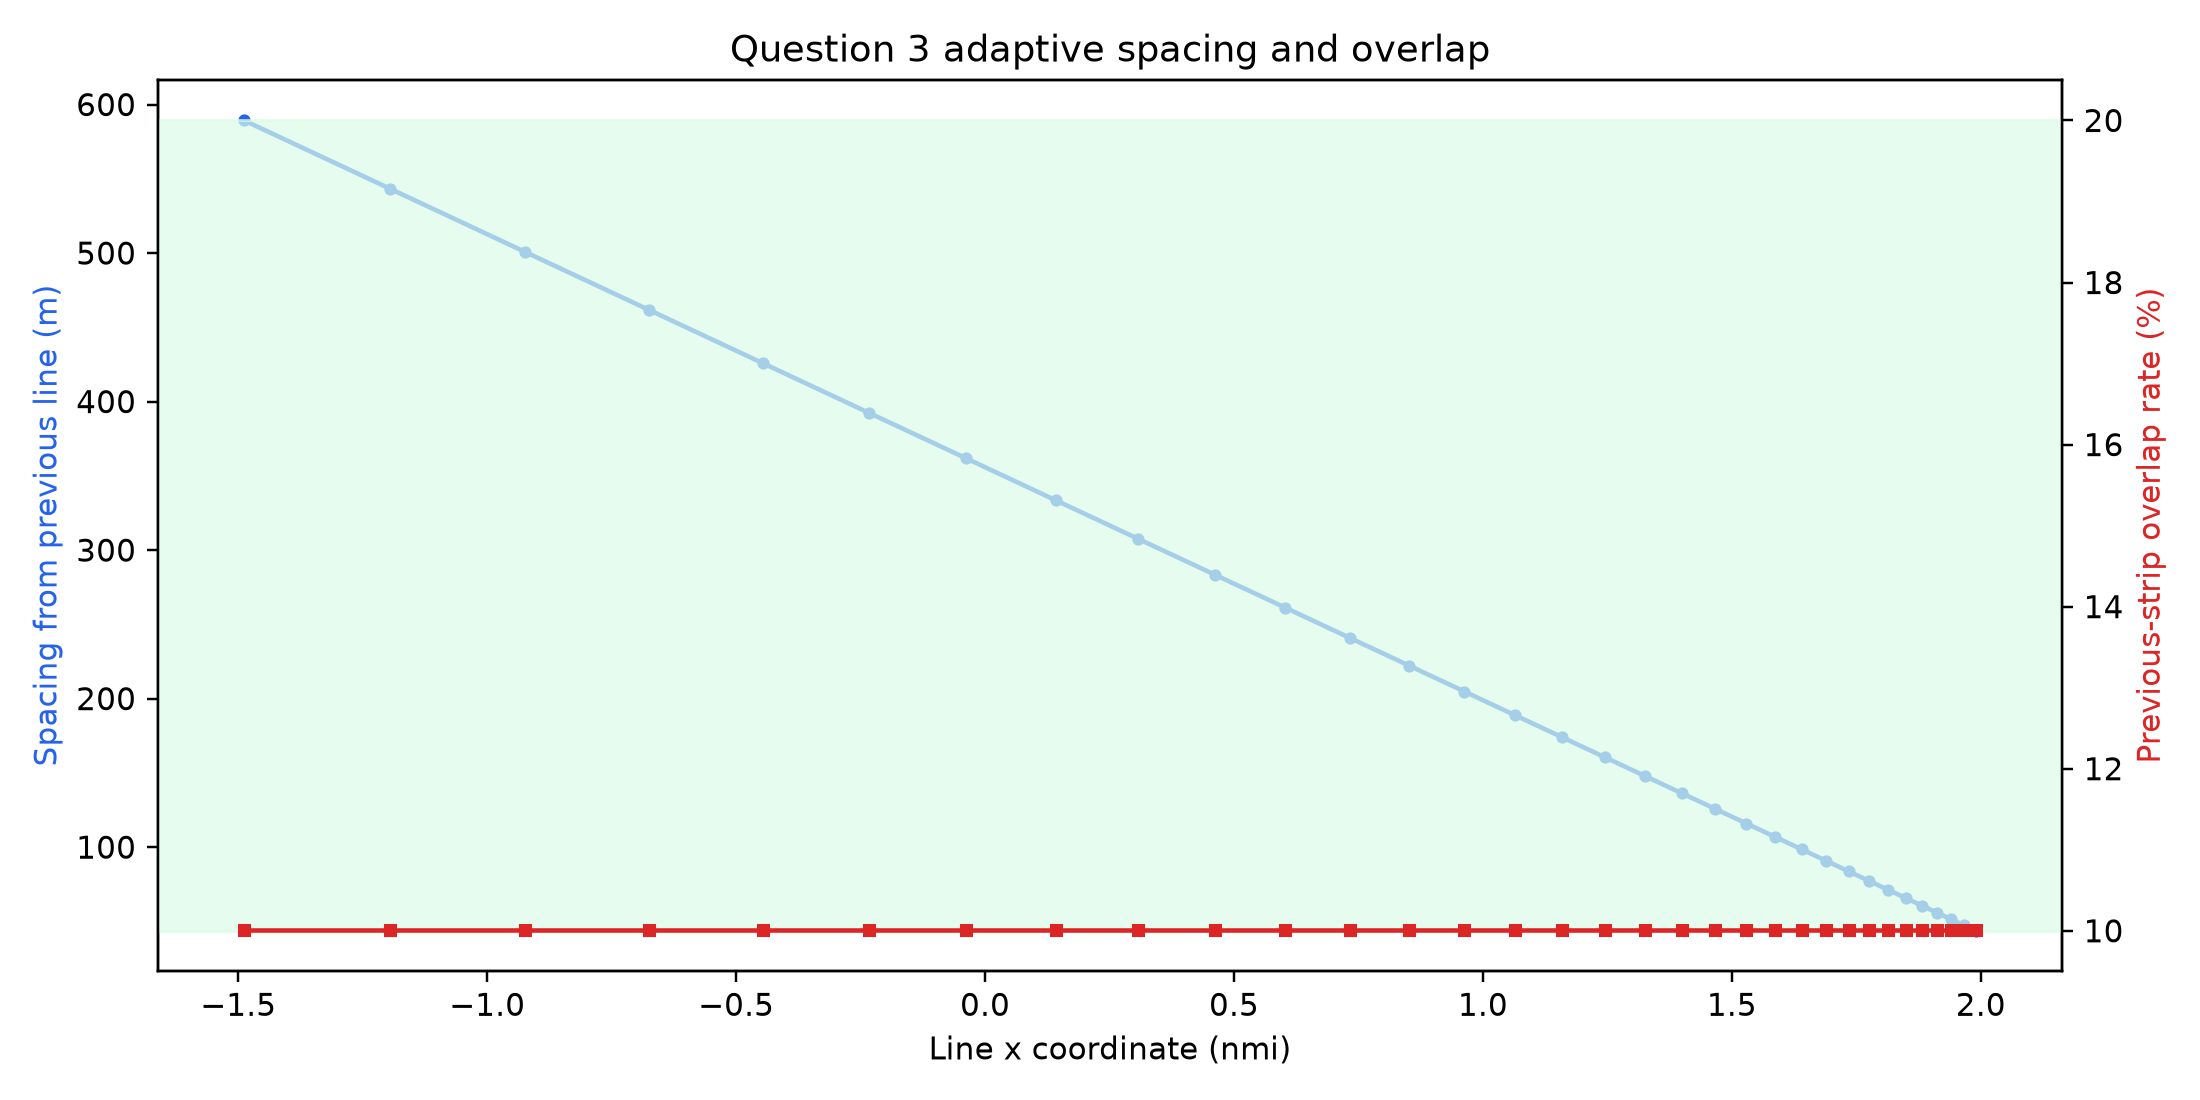
\includegraphics[width=0.88\textwidth]{第3问间距与重叠率-v001.png}
\caption{第3问间距与重叠率}
\label{fig:q3overlap}
\end{figure}

条带并集覆盖全部 $7408\m$ 横向范围，漏测面积为 0；未舍入正式重叠率为 $10.01\%$，当前条带宽度分母下为 $10.8579\%$，仍满足约束。独立射线端点最大差为 $4.55\times10^{-13}\m$。目标重叠率 $10.00\%$、$10.01\%$、$10.10\%$ 均需 34 条，而 $10.50\%$、$15\%$、$20\%$ 分别需 35、36、39 条。相较 $15\%$ 基线的 $133.344\km$，正式方案缩短 $7.408\km$，即 $5.56\%$。最优性仅限等深平行递推类及有限近方向筛查。

\section{第4问：历史网格地形的分块规划}

\subsection{地形模型}

附件网格范围为 $7408\m\times9260\m$，共有 $251\times201$ 个水深节点，水深为 $20.0$--$197.2\m$。主模型采用规则网格单元内的分片双线性函数
\begin{equation}
D(u,v)=(1-u)(1-v)D_{00}+u(1-v)D_{10}+(1-u)vD_{01}+uvD_{11}.
\end{equation}
以 $z=-D$ 表示海底高程，局部坡度为
\begin{equation}
\alpha=\arctan\sqrt{D_x^2+D_y^2}.
\end{equation}
节点最大重建误差为 $5.684\times10^{-14}\m$；坡度中位数为 $0.6189\degree$，最大值为 $3.3719\degree$。另以两种固定对角线的分片三角面作敏感性对照。

\begin{figure}[H]
\centering
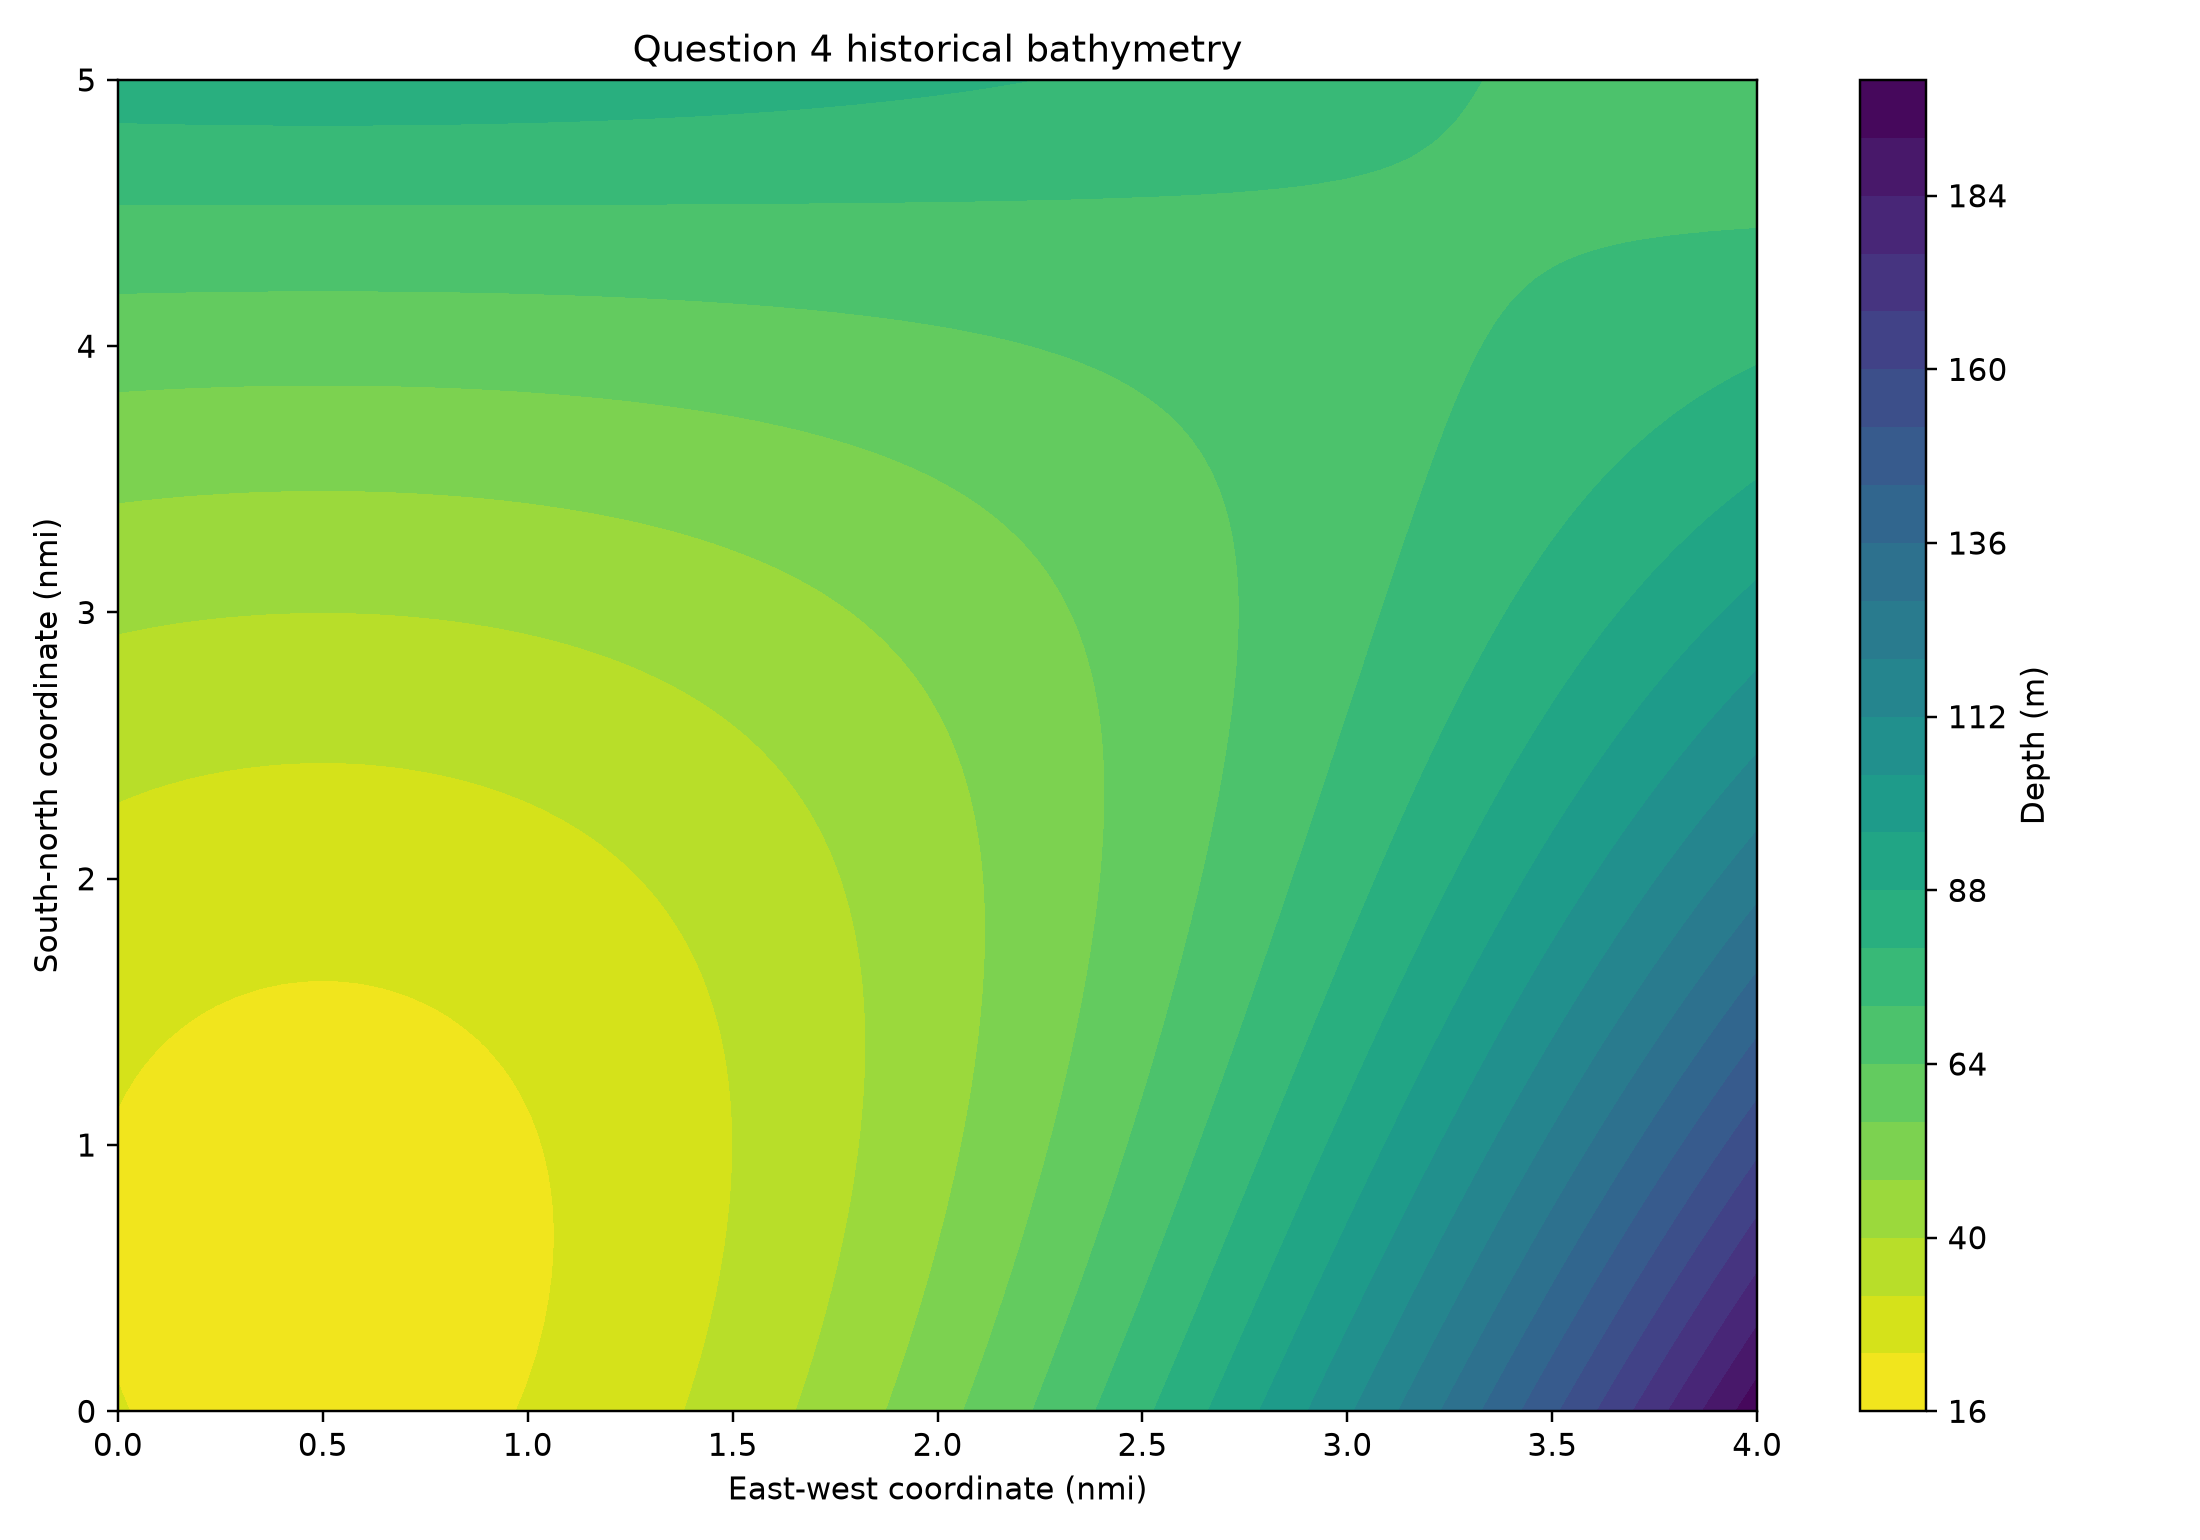
\includegraphics[width=0.82\textwidth]{第4问地形图-v001.png}
\caption{第4问历史水深地形}
\label{fig:q4terrain}
\end{figure}

\begin{figure}[H]
\centering
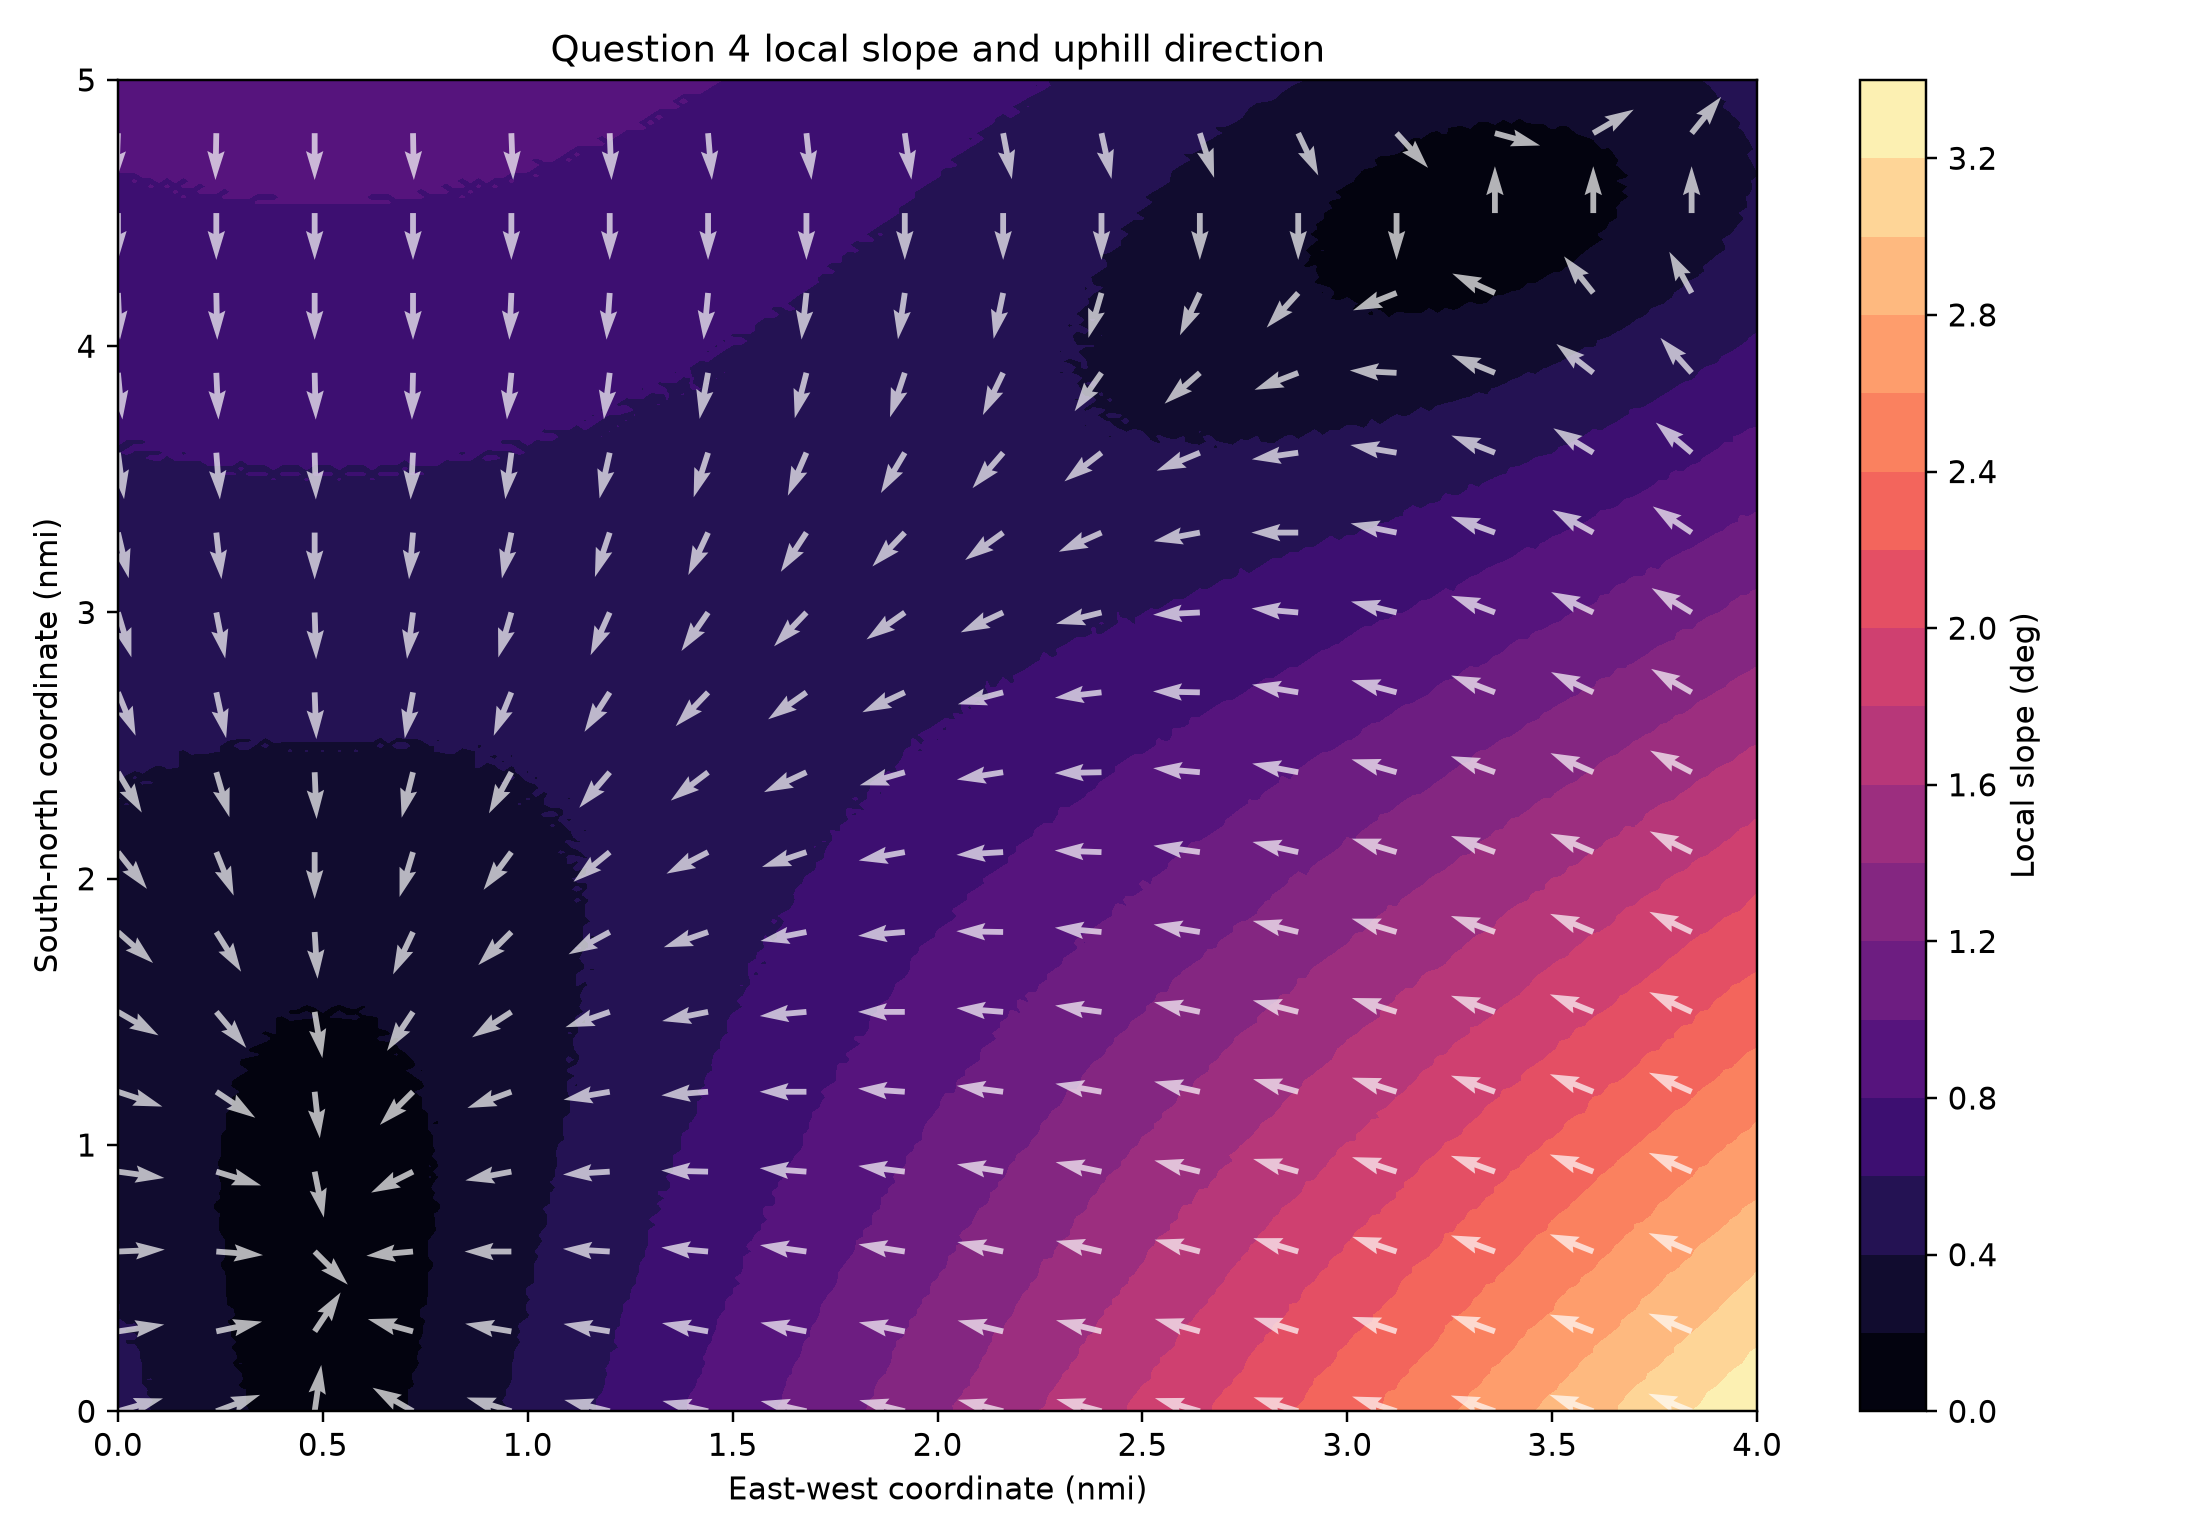
\includegraphics[width=0.82\textwidth]{第4问坡度坡向图-v001.png}
\caption{第4问局部坡度与上坡方向}
\label{fig:q4slope}
\end{figure}

\subsection{局部水平覆盖与三目标}

对局部水深 $D$ 和测线横向高程坡度 $m_\perp$，水平规划域内的左右覆盖距离为
\begin{equation}
w_L=\frac{D\sin\gamma}{\cos\gamma-m_\perp\sin\gamma},\qquad
w_R=\frac{D\sin\gamma}{\cos\gamma+m_\perp\sin\gamma}.
\end{equation}
逐沿线切片合并所有 $[c-w_L,c+w_R]$ 区间，积分未覆盖宽度得到
\begin{equation}
p_{\rm miss}=\frac{A_{\rm miss}}{A_{\rm total}}\times100\%.
\end{equation}

同一分区内按中心坐标递增确定相邻测线，并沿有序相邻对统计
\begin{equation}
\eta_i(s)=\frac{R_{i-1}(s)-L_i(s)}{R_{i-1}(s)-L_{i-1}(s)}>20\%
\end{equation}
的线段长度。分层目标依次最小化漏测率、过度重叠逐对计数长度和区域内测线总长度。

\subsection{候选比较与最终方案}

表\ref{tab:q4candidates} 为 20 m 粗筛结果。统一基线最短但存在 $9.14\%$ 漏测；零漏测候选中，分块方案的过度重叠长度最小。

\begin{table}[H]
\centering
\caption{第4问候选方案比较}
\label{tab:q4candidates}
\begin{tabular}{lrrr}
\toprule
方案 & 漏测率/\% & 过度重叠/km & 总长度/km\\
\midrule
统一纵向等间距 & 9.138880 & 248.820 & 444.480\\
纵向自适应，目标0 & 0 & 279.820 & 555.600\\
纵向自适应，目标1\% & 0 & 292.680 & 564.860\\
纵向自适应，目标2\% & 0 & 294.320 & 564.860\\
纵向自适应，目标5\% & 0 & 321.860 & 583.380\\
纵向自适应，目标10\% & 0 & 383.360 & 620.420\\
横向自适应，目标2\% & 0 & 375.312 & 644.496\\
南北分块两方向 & 0 & 131.312 & 473.186\\
分块并增加修补线 & 0 & 132.794 & 474.668\\
\bottomrule
\end{tabular}
\end{table}

最终在 $y=2.5\nmi$ 处分区：南区布置 59 条南北向线，每条 $4630\m$；北区布置 27 条东西向线，每条 $7408\m$。接口采用半开归属，分区间不构造人为相邻对。共 86 条线，总长度
\begin{equation}
L_4=59\times4630+27\times7408=473186\m=473.186\km.
\end{equation}

\begin{figure}[H]
\centering
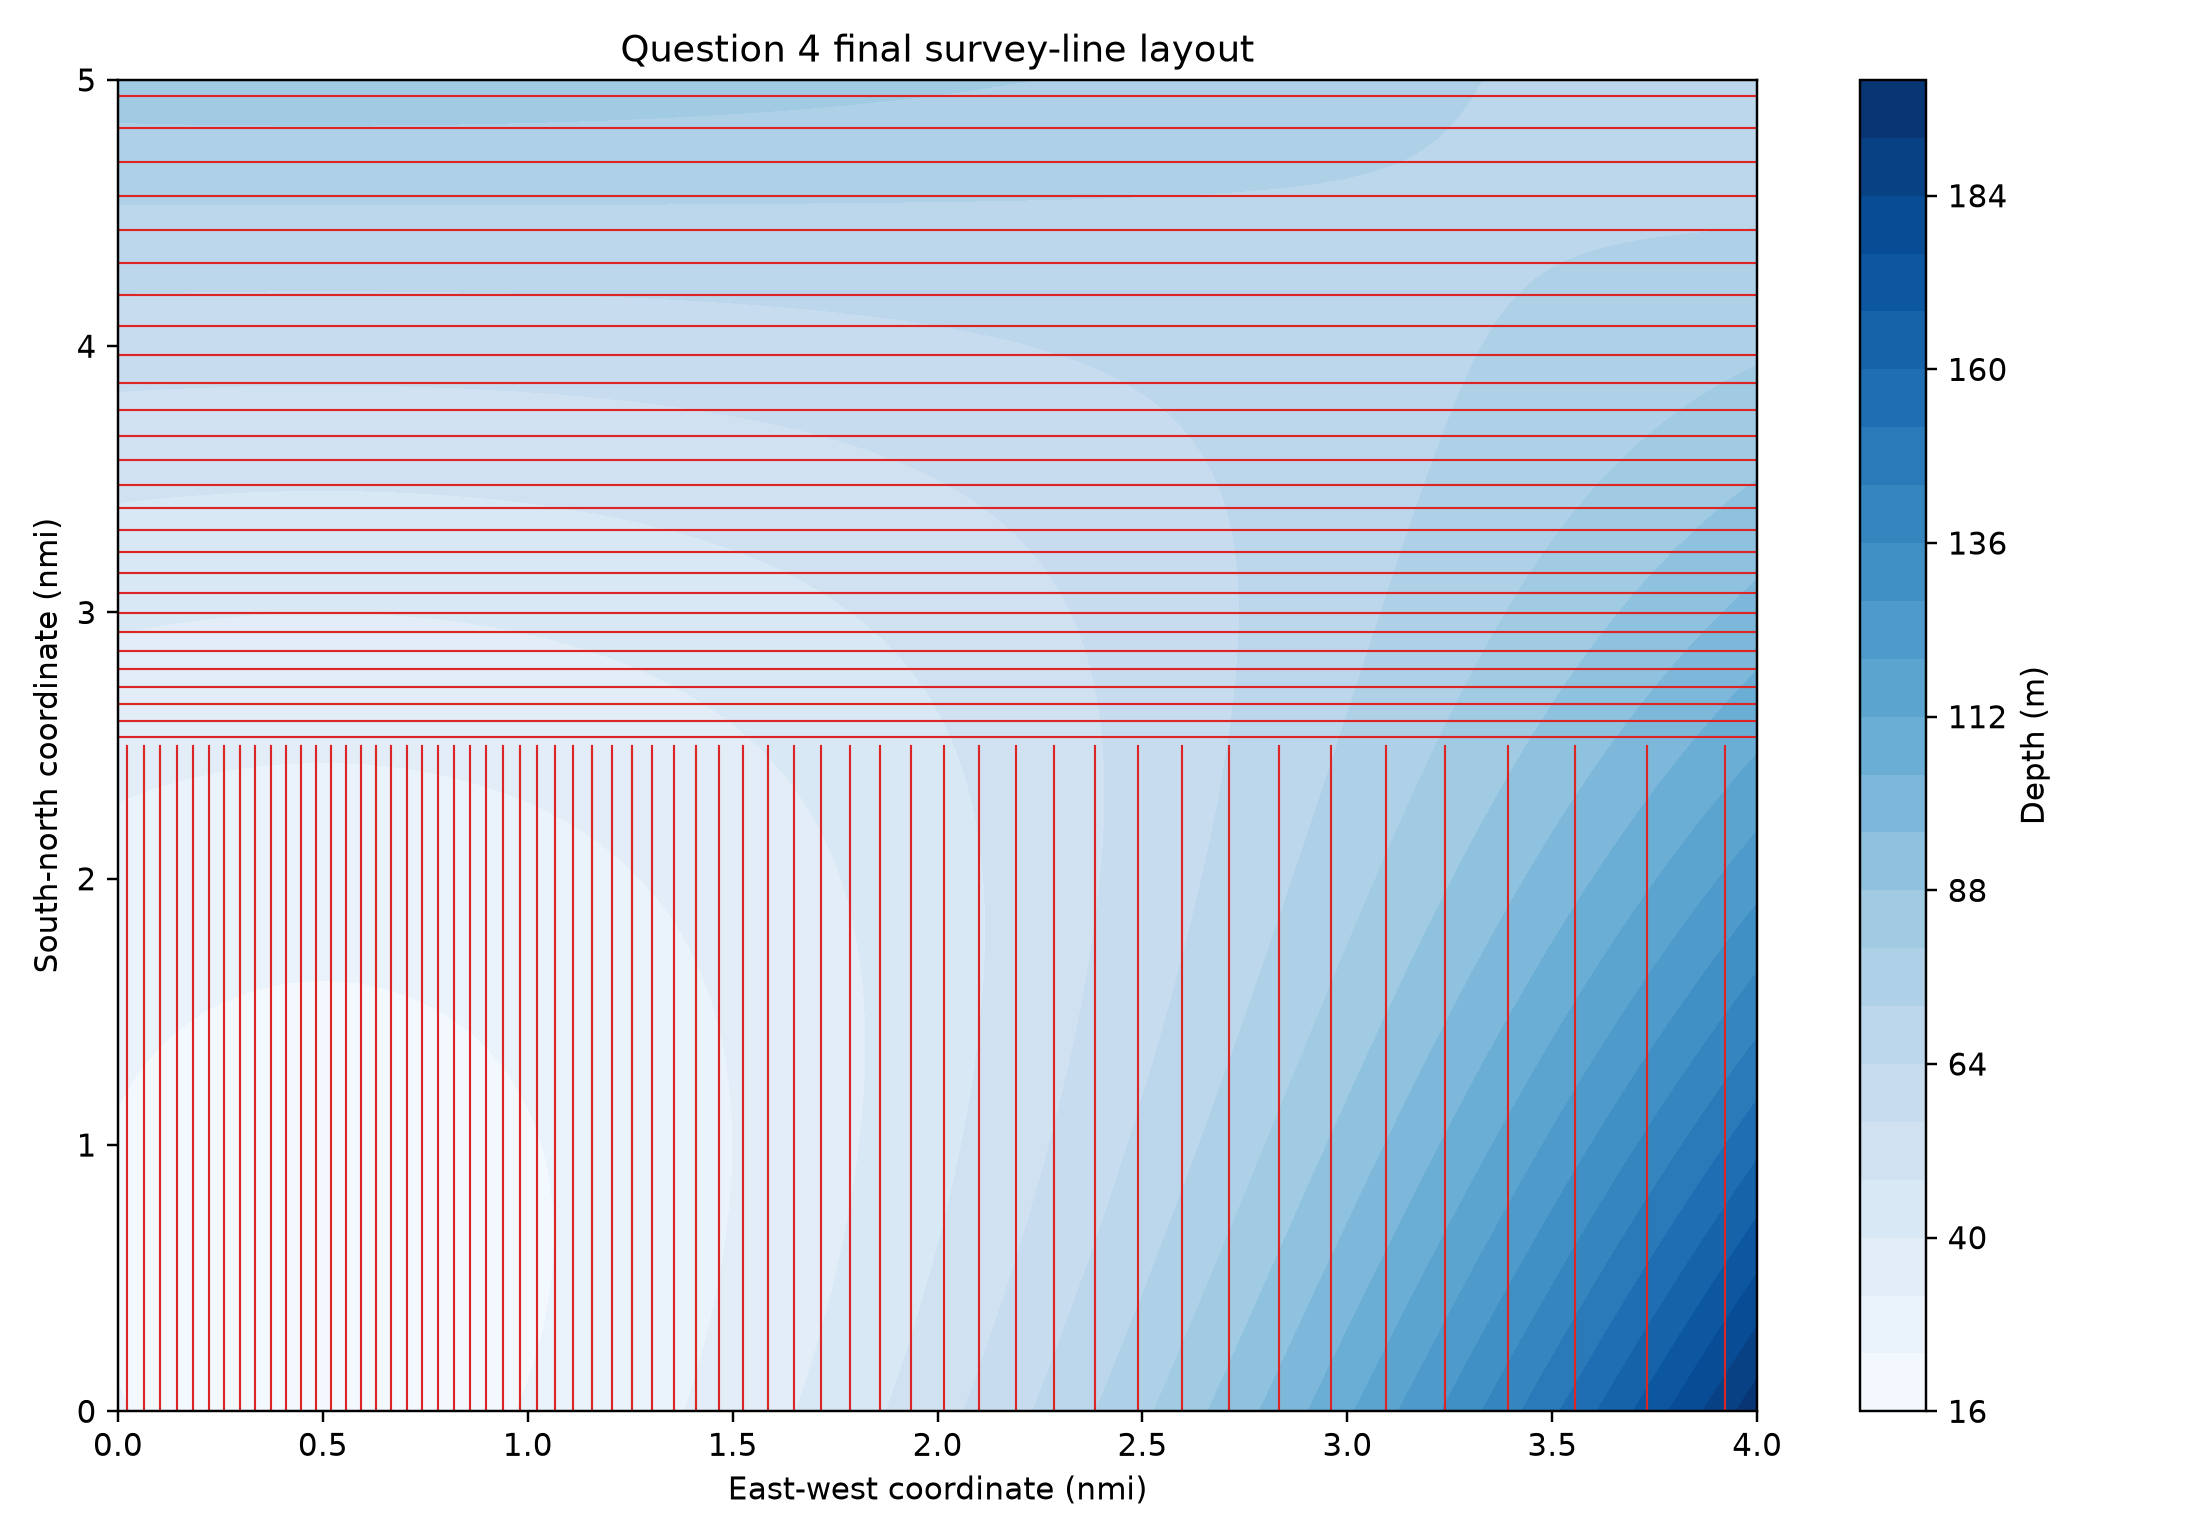
\includegraphics[width=0.82\textwidth]{第4问最终测线布局-v001.png}
\caption{第4问最终测线布局}
\label{fig:q4layout}
\end{figure}

\subsection{三项指标与稳定性}

双线性地形、$5\m$ 主评价下
\begin{equation}
p_{\rm miss}=0\%,\qquad
L_{\eta>20\%}=131287.199730\m\approx131.287\km.
\end{equation}

\begin{figure}[H]
\centering
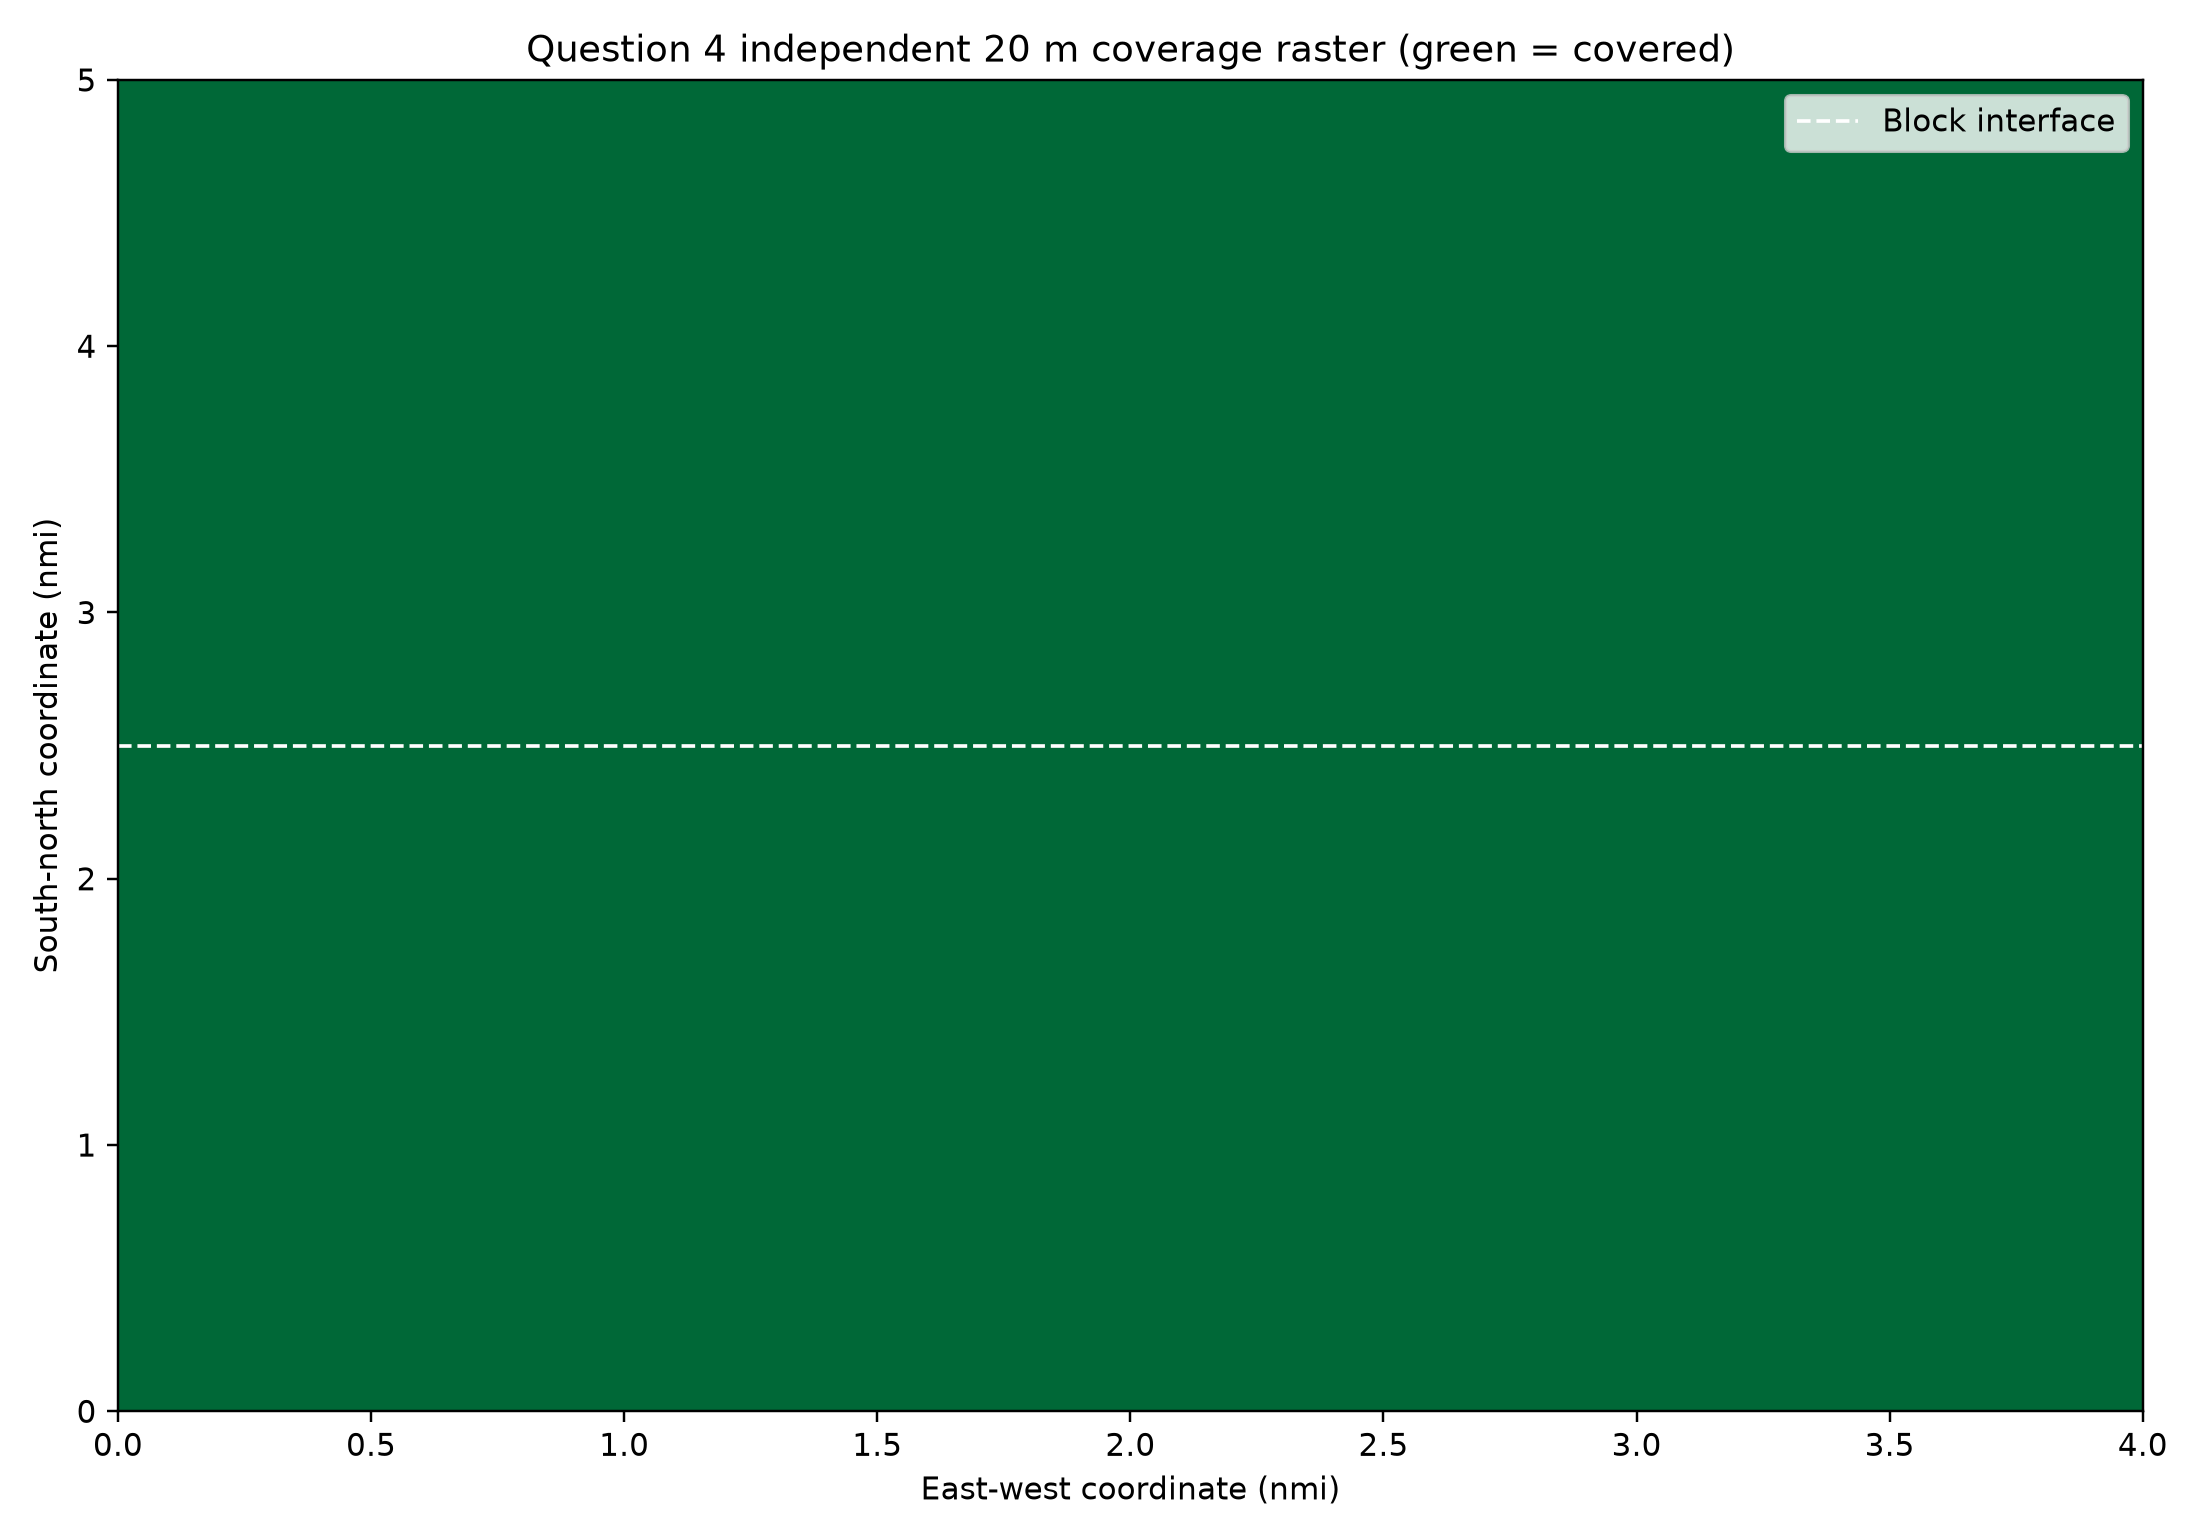
\includegraphics[width=0.82\textwidth]{第4问覆盖与漏测图-v001.png}
\caption{独立20 m覆盖栅格；绿色表示覆盖}
\label{fig:q4coverage}
\end{figure}

\begin{figure}[H]
\centering
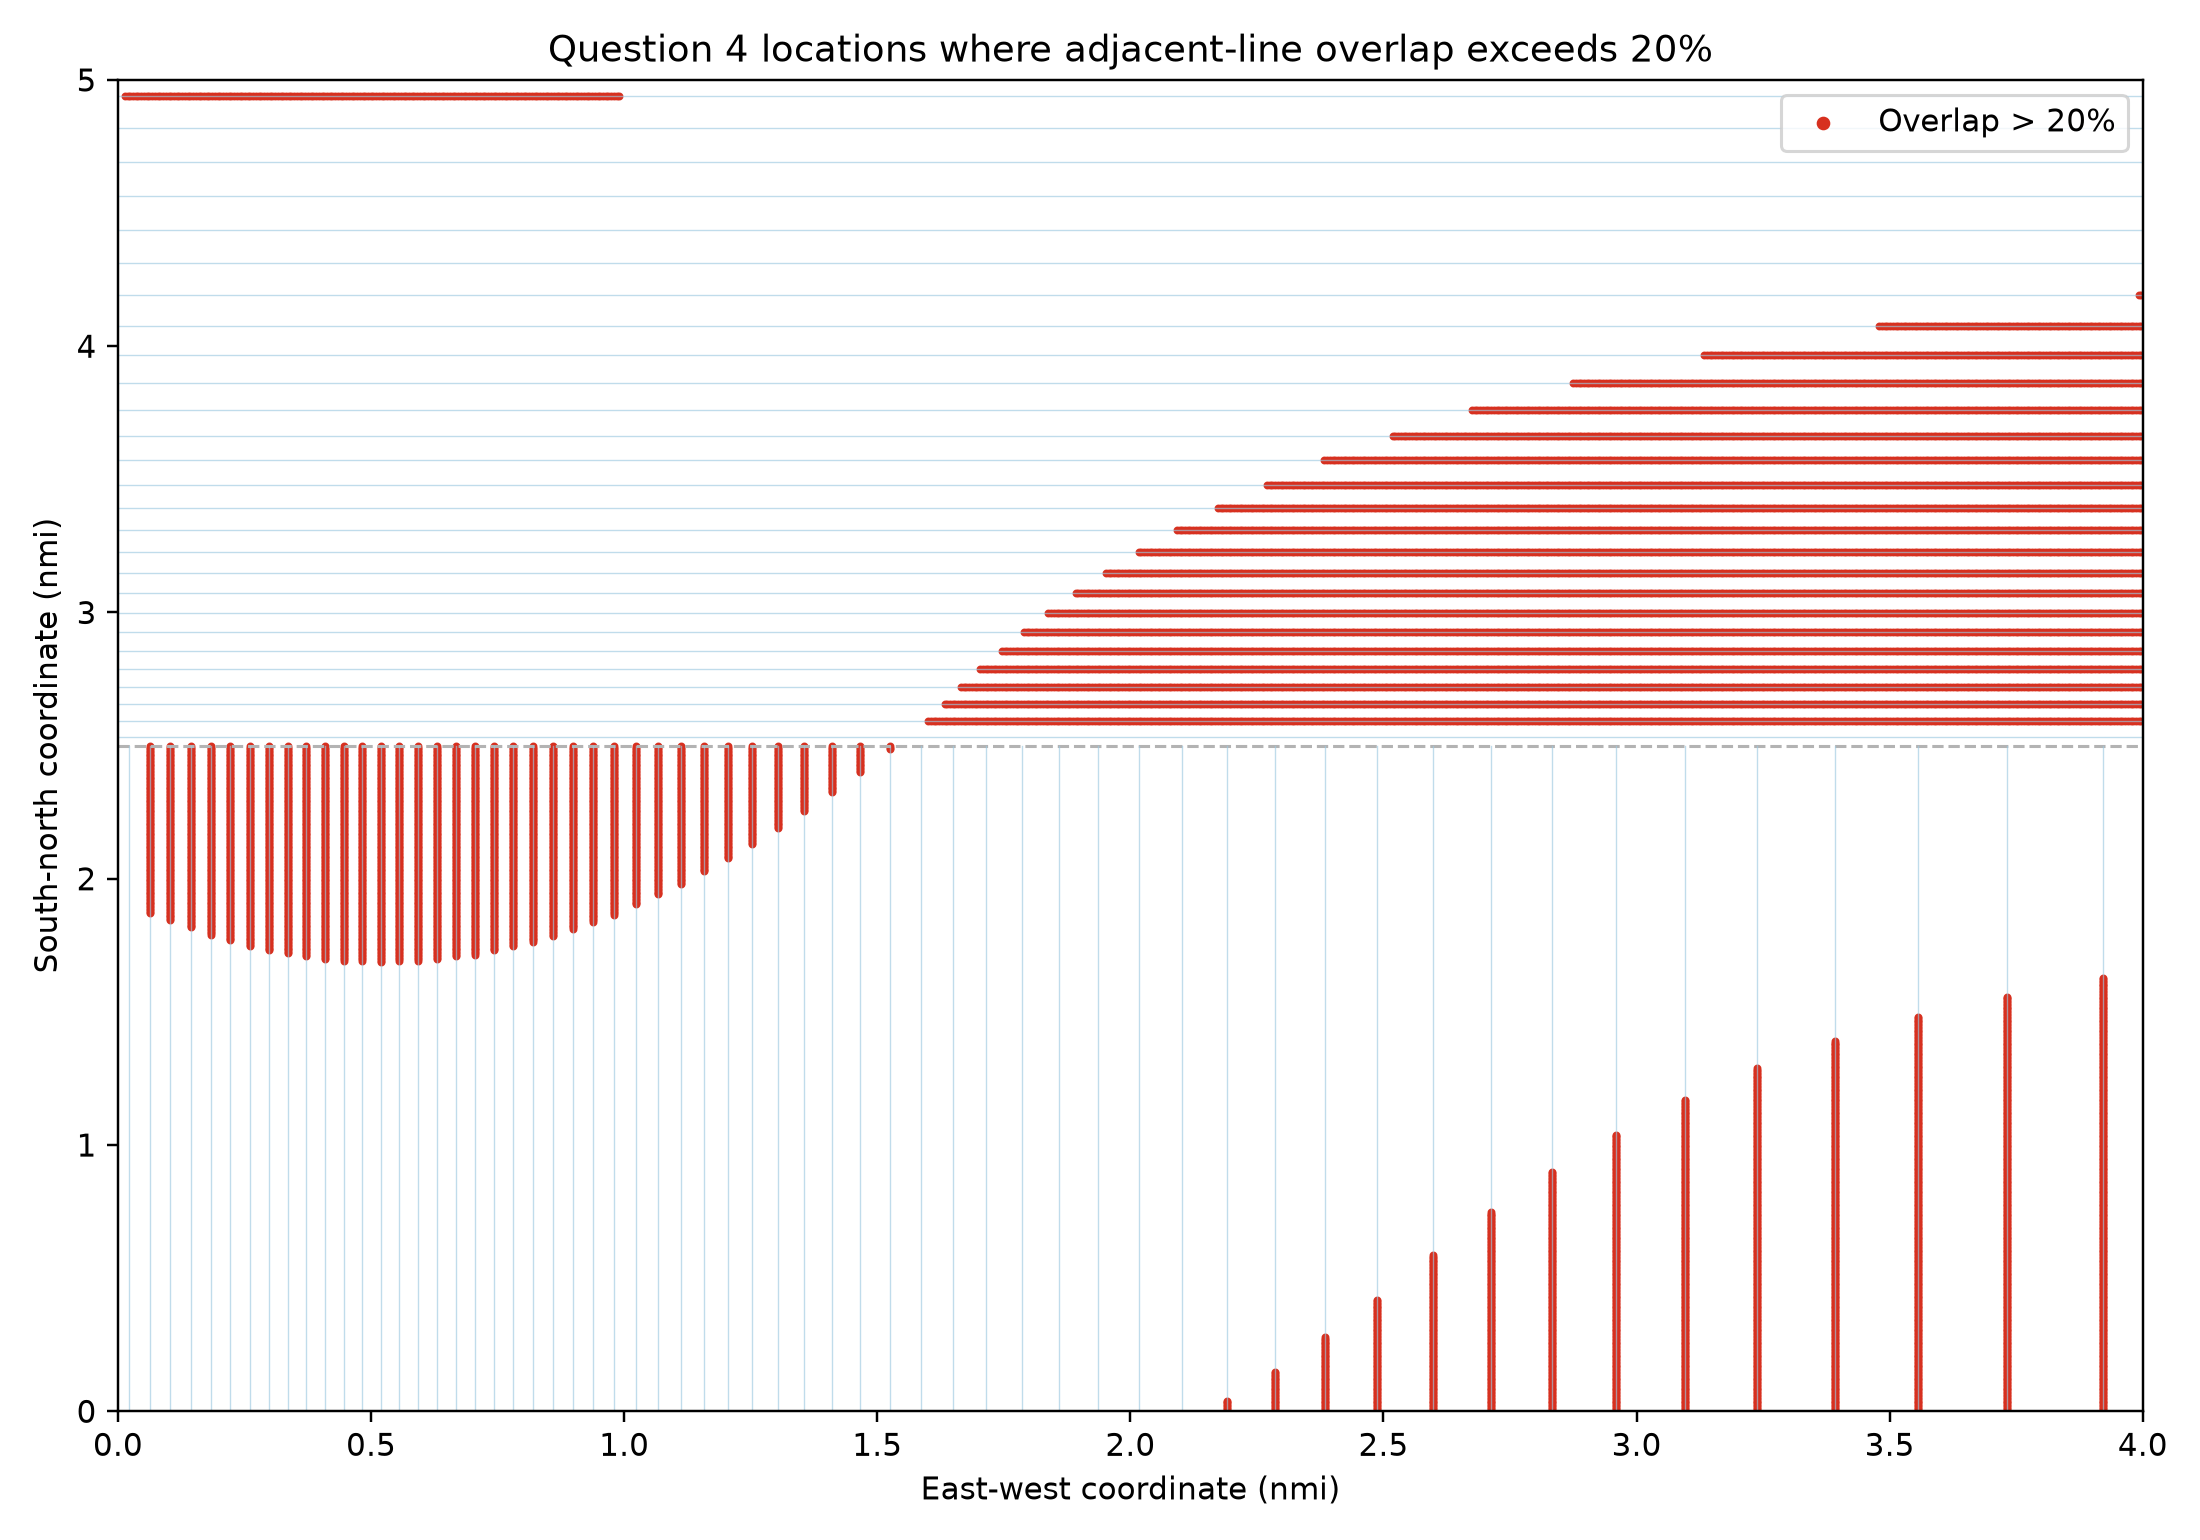
\includegraphics[width=0.82\textwidth]{第4问过度重叠位置-v001.png}
\caption{相邻重叠率超过20\%的位置}
\label{fig:q4overlap}
\end{figure}

\begin{table}[H]
\centering
\caption{第4问分辨率与地形表示敏感性}
\begin{tabular}{lrrr}
\toprule
表示与步长 & 漏测面积/$\mathrm{m}^2$ & 漏测率/\% & 过度重叠/km\\
\midrule
双线性10 m & 0 & 0 & 131.292194\\
双线性5 m & 0 & 0 & 131.287200\\
主对角三角面5 m & 0 & 0 & 131.272201\\
副对角三角面5 m & 0.006571 & $9.5783\times10^{-9}$ & 131.277205\\
\bottomrule
\end{tabular}
\end{table}

独立二维栅格在 10 m 与 5 m 下均无漏测单元；三种 5 m 表示的过度重叠长度位于 $131.272$--$131.287\km$。副对角三角面产生的极小漏测说明结果宜表述为“规划分辨率下近零漏测”。人工平坦地形、100 组随机单平面、第2问公式退化、边界裁剪、相邻关系、总长度重算和工作簿读回均通过。

\section{模型评价}

\subsection{优点}
\begin{enumerate}[leftmargin=2.6em]
  \item 四问共享总开角 $\theta$、半开角 $\gamma$ 与方向角 $\beta$，并明确坡面宽度和水平投影宽度的关系。
  \item 有向重叠率保留漏测信息，条带并集直接验证边界与全区域覆盖。
  \item 第2、3问使用独立射线求交；第4问冻结后另用独立栅格、人工地形和两种三角剖分验证。
  \item 候选选择采用预先登记的分层目标，不以事后任意权重制造结论。
  \item 逐线工作簿、JSON、代码与图件形成可追溯复现链。
\end{enumerate}

\subsection{局限}
\begin{enumerate}[leftmargin=2.6em]
  \item 未考虑声速折射、船体姿态、定位、设备标定与波束脚印厚度。
  \item 第4问以历史网格为规划基准，实际作业需最新复测和安全裕度。
  \item 第3、4问不计转场与转弯，因此总长度不是完整航行里程。
  \item 第3问最优性限于等深平行递推类和有限近方向筛查；第4问限于实际计算的九个有限直线/分块候选。
  \item 分辨率和三角剖分差异只刻画数值表示敏感性，不能替代物理不确定性分析。
\end{enumerate}

\section{结论}

本文建立了从二维恒坡、三维方向到矩形覆盖和规则网格地形的统一多波束模型。第一问完成表1并识别浅水侧漏测；第二问完成 64 个方向—距离组合并通过三维独立求交；第三问用 34 条南北向变间距测线得到 $125.936\km$ 的全覆盖方案，正式重叠率为 $10.01\%$；第四问用 86 条分块直线得到 $473.186\km$ 的规划方案，5 m 主模型漏测率为 0，过度重叠逐对计数总长约 $131.287\km$。所有正式数字均来自未舍入计算和版本化结果文件，验证证据支持其在所声明模型和候选范围内成立。

\section{参考资料说明}

盲解期间未访问互联网、外部论文、题解或远程代码库。方法依据仅为匿名工作区中已审核固定版本的本地方法卡，包括事实—假设—单位与复现接口、二维射线与有向坡度、三维射线与方向投影、区间覆盖与重叠、条带区域覆盖优化、规则网格地形与区域测度、数值验证与稳定性。具体文件版本与 SHA-256 记录在工作区的《方法库查阅记录》中。

\appendix
\section{正式结果与复现文件}

第1问正式文件为根目录 \texttt{result1.xlsx}；第2问为 \texttt{result2.xlsx}；第3问和第4问的逐线清单分别位于 \texttt{工作记录/结果/Q03} 与 \texttt{工作记录/结果/Q04}。各问模型脚本、独立验证、诊断 JSON、图件、结果哈希及正文证据映射均保存在 \texttt{工作记录} 下的版本化目录。完整运行顺序见同目录《可复现说明-v001.md》。

\end{document}
